\documentclass{article}
%--PASTE INTO MAIN FILE--
% \documentclass{article}
% %--PASTE INTO MAIN FILE--
% \documentclass{article}
% %--PASTE INTO MAIN FILE--
% \documentclass{article}
% \input{TexBase/DocumentBase.tex}
% \end{document}

\usepackage[margin = 0.7in]{geometry}
\usepackage{graphicx}
\usepackage{graphics}
\usepackage[T1]{fontenc}
\usepackage[polish]{babel}
\usepackage{cmap}
\usepackage[utf8]{inputenc}
\usepackage{float}
\usepackage{tabularx}
\usepackage[table,xcdraw]{xcolor}
\usepackage{lipsum}
\usepackage{titlesec}
\usepackage{minted}
\usepackage{xcolor}
\usepackage{caption}
\usepackage{enumitem}
\usepackage{csvsimple}
\usepackage{natbib}
\usepackage{blindtext}

\usepackage{amsmath} %math

\usepackage{numprint} % rounding
\usepackage[round-precision=3,round-mode=figures, scientific-notation=true]{siunitx} %scientific notation

\usepackage[hidelinks]{hyperref}
\usepackage{url}

\usepackage{bm} %bold for math


%TABS
\usepackage[]{booktabs}
\usepackage{tabularray}
\usepackage{multirow}

%\title{}
\author{Michał Dziedziak}
\date{\today}


\titlespacing\section{0pt}{12pt plus 4pt minus 2pt}{0pt plus 2pt minus 2pt}
\titlespacing\subsection{0pt}{12pt plus 4pt minus 2pt}{0pt plus 2pt minus 2pt}
\titlespacing\subsubsection{0pt}{12pt plus 4pt minus 2pt}{0pt plus 2pt minus 2pt}
\setlength{\parskip}{\baselineskip}%
\setlength{\parindent}{0pt}%

\newcommand{\squeezeup}{\vspace{-5mm}}


\begin{document}

\begin{titlepage}
    \begin{center}
        \vspace*{5cm}
        \rule{500pt}{1pt}\\
        \vspace*{0.5cm}
        \LARGE
        \textbf{Inżyniera Obrazów}\\
        \Large
        Laboratorium numer 2
        \vspace*{0.5cm}
        \rule{500pt}{1pt}
    \end{center}

    \vspace*{10cm}

    {\raggedright
        \large
        \textbf{Autor sprawozdania:} Michał Dziedziak 263901\\
        \textbf{Imię i Nazwisko prowadzącego kurs:} dr inż. Jan Nikodem\\
        \textbf{Dzień i godzina zajęć:} czwartek, 11:15 - 14:15
    }
\end{titlepage}


\tableofcontents
% \listoftables

%\renewcommand\listoflistingscaption{List of source codes}
% \listoflistings

\listoffigures


\newpage


% \begin{table}[H]
%     \centering
%     \begin{tabular}{|c|c|c|c|}%
%         \hline
%         \bfseries Numer iteracji & \bfseries Czas zalezienia rozwiązania [ms] & Koszt ścieżki & Błąd względny% specify table head
%         \csvreader[head to column names]{Csv/BestPathTest_SimulatedAnnealing_LINEAR_ftv47.csv}{}% use head of csv as column names
%         {\\\hline\Iteration & \num{\TimeInMiliSeconds} & \Cost & \num[round-precision=2, round-mode=places, scientific-notation=false]{\Error}\%}% specify your columns here
%         \\\hline    
%     \end{tabular}
%     \caption{}
%     \label{tab:}
% \end{table}

% \begin{figure}[H]
%     \centering
%     \resizebox{\columnwidth}{!}{%
%     \includegraphics{}%
%     }
%     \caption{}
%     \label{fig:}
% \end{figure}

% \begin{listing}[H]
%     \begin{minted}[frame=single,framesep=2mm,linenos,fontsize=\footnotesize]{language}
%         some code
%     \end{minted}
%     \caption{}
%     \label{lst:}
% \end{listing}


% \bibliographystyle{plainnat}
% \bibliography{TexBase/Bibliography}

% \end{document}

\usepackage[margin = 0.7in]{geometry}
\usepackage{graphicx}
\usepackage{graphics}
\usepackage[T1]{fontenc}
\usepackage[polish]{babel}
\usepackage{cmap}
\usepackage[utf8]{inputenc}
\usepackage{float}
\usepackage{tabularx}
\usepackage[table,xcdraw]{xcolor}
\usepackage{lipsum}
\usepackage{titlesec}
\usepackage{minted}
\usepackage{xcolor}
\usepackage{caption}
\usepackage{enumitem}
\usepackage{csvsimple}
\usepackage{natbib}
\usepackage{blindtext}

\usepackage{amsmath} %math

\usepackage{numprint} % rounding
\usepackage[round-precision=3,round-mode=figures, scientific-notation=true]{siunitx} %scientific notation

\usepackage[hidelinks]{hyperref}
\usepackage{url}

\usepackage{bm} %bold for math


%TABS
\usepackage[]{booktabs}
\usepackage{tabularray}
\usepackage{multirow}

%\title{}
\author{Michał Dziedziak}
\date{\today}


\titlespacing\section{0pt}{12pt plus 4pt minus 2pt}{0pt plus 2pt minus 2pt}
\titlespacing\subsection{0pt}{12pt plus 4pt minus 2pt}{0pt plus 2pt minus 2pt}
\titlespacing\subsubsection{0pt}{12pt plus 4pt minus 2pt}{0pt plus 2pt minus 2pt}
\setlength{\parskip}{\baselineskip}%
\setlength{\parindent}{0pt}%

\newcommand{\squeezeup}{\vspace{-5mm}}


\begin{document}

\begin{titlepage}
    \begin{center}
        \vspace*{5cm}
        \rule{500pt}{1pt}\\
        \vspace*{0.5cm}
        \LARGE
        \textbf{Inżyniera Obrazów}\\
        \Large
        Laboratorium numer 2
        \vspace*{0.5cm}
        \rule{500pt}{1pt}
    \end{center}

    \vspace*{10cm}

    {\raggedright
        \large
        \textbf{Autor sprawozdania:} Michał Dziedziak 263901\\
        \textbf{Imię i Nazwisko prowadzącego kurs:} dr inż. Jan Nikodem\\
        \textbf{Dzień i godzina zajęć:} czwartek, 11:15 - 14:15
    }
\end{titlepage}


\tableofcontents
% \listoftables

%\renewcommand\listoflistingscaption{List of source codes}
% \listoflistings

\listoffigures


\newpage


% \begin{table}[H]
%     \centering
%     \begin{tabular}{|c|c|c|c|}%
%         \hline
%         \bfseries Numer iteracji & \bfseries Czas zalezienia rozwiązania [ms] & Koszt ścieżki & Błąd względny% specify table head
%         \csvreader[head to column names]{Csv/BestPathTest_SimulatedAnnealing_LINEAR_ftv47.csv}{}% use head of csv as column names
%         {\\\hline\Iteration & \num{\TimeInMiliSeconds} & \Cost & \num[round-precision=2, round-mode=places, scientific-notation=false]{\Error}\%}% specify your columns here
%         \\\hline    
%     \end{tabular}
%     \caption{}
%     \label{tab:}
% \end{table}

% \begin{figure}[H]
%     \centering
%     \resizebox{\columnwidth}{!}{%
%     \includegraphics{}%
%     }
%     \caption{}
%     \label{fig:}
% \end{figure}

% \begin{listing}[H]
%     \begin{minted}[frame=single,framesep=2mm,linenos,fontsize=\footnotesize]{language}
%         some code
%     \end{minted}
%     \caption{}
%     \label{lst:}
% \end{listing}


% \bibliographystyle{plainnat}
% \bibliography{TexBase/Bibliography}

% \end{document}

\usepackage[margin = 0.7in]{geometry}
\usepackage{graphicx}
\usepackage{graphics}
\usepackage[T1]{fontenc}
\usepackage[polish]{babel}
\usepackage{cmap}
\usepackage[utf8]{inputenc}
\usepackage{float}
\usepackage{tabularx}
\usepackage[table,xcdraw]{xcolor}
\usepackage{lipsum}
\usepackage{titlesec}
\usepackage{minted}
\usepackage{xcolor}
\usepackage{caption}
\usepackage{enumitem}
\usepackage{csvsimple}
\usepackage{natbib}
\usepackage{blindtext}

\usepackage{amsmath} %math

\usepackage{numprint} % rounding
\usepackage[round-precision=3,round-mode=figures, scientific-notation=true]{siunitx} %scientific notation

\usepackage[hidelinks]{hyperref}
\usepackage{url}

\usepackage{bm} %bold for math


%TABS
\usepackage[]{booktabs}
\usepackage{tabularray}
\usepackage{multirow}

%\title{}
\author{Michał Dziedziak}
\date{\today}


\titlespacing\section{0pt}{12pt plus 4pt minus 2pt}{0pt plus 2pt minus 2pt}
\titlespacing\subsection{0pt}{12pt plus 4pt minus 2pt}{0pt plus 2pt minus 2pt}
\titlespacing\subsubsection{0pt}{12pt plus 4pt minus 2pt}{0pt plus 2pt minus 2pt}
\setlength{\parskip}{\baselineskip}%
\setlength{\parindent}{0pt}%

\newcommand{\squeezeup}{\vspace{-5mm}}


\begin{document}

\begin{titlepage}
    \begin{center}
        \vspace*{5cm}
        \rule{500pt}{1pt}\\
        \vspace*{0.5cm}
        \LARGE
        \textbf{Inżyniera Obrazów}\\
        \Large
        Laboratorium numer 2
        \vspace*{0.5cm}
        \rule{500pt}{1pt}
    \end{center}

    \vspace*{10cm}

    {\raggedright
        \large
        \textbf{Autor sprawozdania:} Michał Dziedziak 263901\\
        \textbf{Imię i Nazwisko prowadzącego kurs:} dr inż. Jan Nikodem\\
        \textbf{Dzień i godzina zajęć:} czwartek, 11:15 - 14:15
    }
\end{titlepage}


\tableofcontents
% \listoftables

%\renewcommand\listoflistingscaption{List of source codes}
% \listoflistings

\listoffigures


\newpage


% \begin{table}[H]
%     \centering
%     \begin{tabular}{|c|c|c|c|}%
%         \hline
%         \bfseries Numer iteracji & \bfseries Czas zalezienia rozwiązania [ms] & Koszt ścieżki & Błąd względny% specify table head
%         \csvreader[head to column names]{Csv/BestPathTest_SimulatedAnnealing_LINEAR_ftv47.csv}{}% use head of csv as column names
%         {\\\hline\Iteration & \num{\TimeInMiliSeconds} & \Cost & \num[round-precision=2, round-mode=places, scientific-notation=false]{\Error}\%}% specify your columns here
%         \\\hline    
%     \end{tabular}
%     \caption{}
%     \label{tab:}
% \end{table}

% \begin{figure}[H]
%     \centering
%     \resizebox{\columnwidth}{!}{%
%     \includegraphics{}%
%     }
%     \caption{}
%     \label{fig:}
% \end{figure}

% \begin{listing}[H]
%     \begin{minted}[frame=single,framesep=2mm,linenos,fontsize=\footnotesize]{language}
%         some code
%     \end{minted}
%     \caption{}
%     \label{lst:}
% \end{listing}


% \bibliographystyle{plainnat}
% \bibliography{TexBase/Bibliography}



\section{Temat laboratorium}
W ramach trzecich zajęć laboratoryjnych mieliśmy wykonać zadanie 4 i 5 z listy drugiej.
Punkty te dotyczyły implementacji algorytmu JPEG.


\section{Zadania do wykonania i plan pracy}

\subsection{Zadanie 4: Implementacja części algorytmu JPEG}
Zadanie czwarte zakładało uproszczoną implementację algorytmu JPEG. W ramach tego punktu mieliśmy
zaimplementować:
\begin{itemize}
    \item Kroki: 0, 1, 2, 3, 7, 8 algorytmu JPEG. Gdzie:
          \begin{itemize}
              \item Krok 0: Wczytanie obrazu wejściowego,
              \item Krok 1: Konwersja modelu barw: RGB -> YCbCr,
              \item Krok 2: Przeskalowanie w dół macierzy składowych Cb i Cr,
              \item Krok 3: Podział obrazu na bloki o rozmiarze 8x8,
              \item Krok 7: Zwinięcie każdego bloku 8x8 do wiersza 1x64 - algorytm ZigZag,
              \item Krok 8: Zakodowanie danych obrazu,
          \end{itemize}
    \item Zmierzyć liczbę bajtów powstałego obrazu po kroku 8
    \item Ocenić wpływ kroku 2-go na rozmiar i wygląd, poprzez stworzenie trzech wariancji obrazu:
          \begin{itemize}
              \item bez próbkowania,
              \item z próbkowaniem co drugi element,
              \item z próbkowaniem co czwarty element.
          \end{itemize}
    \item Dokonać dekompresji poprzez odwrócenie powyższych kroków.
\end{itemize}

\subsection{Zadanie 5: Dokończenie implementacji algorytmu JPEG}
Zadanie piąte zakładało dokończenie implementacji algorytmu JPEG. W ramach tego punktu mieliśmy
zaimplementować:
\begin{itemize}
    \item Pozostałe kroki algorytmu:
          \begin{itemize}
              \item Krok 4: Wykonanie dyskretnej transformacji cosinusowej na każdym bloku obrazu,
              \item Krok 5: Podzielenie każdego bloku obrazu przez macierz kwantyzacji,
              \item Krok 6: Zaokrąglenie wartości w każdym bloku do liczb całkowitych.
          \end{itemize}
    \item Ocenić jak wybór czynnika QF (quality factor) wpływa na rozmiar i wygląd obrazka.
    \item Dokonać dekompresji poprzez odwrócenie powyższych kroków.
\end{itemize}

\section{Teoria}

Format JPEG (ang. Joint Photographic Experts Group) jest powszechnie stosowanym standardem kompresji
stratnej do obrazów cyfrowych. Algorytm JPEG składa się z kilku etapów, które pozwalają na efektywną
redukcję rozmiaru pliku przy minimalnej utracie jakości obrazu.

Algorytm JPEG jest symetryczny, co oznacza, że dekompresja jest procesem odwrotnym do kompresji
(dokonuję jej się poprzez odwrócenie kolejności kroków kompresji).


\subsection{Konwersja modelu barw RGB do YCbCr}
W pierwszym kroku obraz jest konwertowany z modelu barw RGB do przestrzeni barw YCbCr. Model YCbCr składa
się z trzech składowych: Y (luminancja), Cb (chrominancja niebieska) i Cr (chrominancja czerwona).
Konwersja ta pozwala na oddzielenie informacji o jasności od informacji o barwie, co ułatwia dalszą kompresję.

\subsection{Przeskalowanie w dół (downsampling) macierzy składowych Cb i Cr}
\subsection{Przeskalowanie w dół (downsampling) macierzy składowych Cb i Cr}
Kolejnym krokiem jest przeskalowanie macierzy składowych Cb i Cr, które odpowiadają za informacje o barwie,
przy użyciu technik próbkowania, takich jak próbkowanie co drugi element lub co czwarty element.
To przeskalowanie pozwala na zmniejszenie rozmiaru danych.

\subsection{Podział obrazu na bloki o rozmiarze 8x8}
Obraz jest dzielony na niewielkie bloki o stałym rozmiarze 8 na 8 pikseli. Ten krok umożliwia stosowanie
transformacji i kwantyzacji na mniejszych fragmentach obrazu, co ułatwia kompresję.

\subsection{Wykonanie dyskretnej transformacji kosinusowej (DCT)} %?? verify
Każdy blok pikseli jest poddawany dyskretnej transformacji kosinusowej.
DCT zamienia blok pikseli na zestaw współczynników reprezentujących jego składowe częstotliwości.
Współczynniki te są obliczane za pomocą następującego równania:

\begin{equation}
    F(u,v) = \frac{2}{\sqrt{MN}} C(u) C(v) \sum_{m=0}^{m-1} \sum_{n=0}^{n-1} f(m,n) \cos \left( \frac{(2m+1)u\pi}{2M} \right) \cos \left( \frac{(2n+1)v\pi}{2N} \right)
\end{equation}
gdzie:
\begin{itemize}
    \item $C(u,v)= \frac{1}{\sqrt{2}}$ dla $u,v$ = 0, w przeciwnym wypadku $C(u,v)=1$
    \item $M$ - ilość wierszy w wejściowym zestawie danych
    \item $N$ - ilość kolumn w wejściowym zestawie danych
    \item $m$ - indeksy próbek z wiersza w domenie przestrzeni, gdzie $0\leq m\leq M-1$
    \item $n$ - indeksy próbek z kolumny w domenie przestrzeni, gdzie $0\leq n\leq N-1$
    \item $f(m,n)$ - wartości przestrzenne w bloku danych wejściowych
    \item $u$ - indeks wiersza w domenie częstotliwości
    \item $v$ - indeks kolumny w domenie częstotliwości
    \item $F(u,v)$ - współczynniki transformaty w domenie częstotliwości
\end{itemize}

Przy założeniu, że $M =N = 8$ równanie przyjmuje postać:
\begin{equation}
    F(u,v) = \frac{C(v)}{2}\sum_{n=0}^{7}\left[\frac{C(u)}{2} \sum_{m=0}^{7}f(m,n)\cos \left( \frac{(2m+1)u\pi}{16} \right) \right] \cos \left( \frac{(2n+1)v\pi}{16} \right)
\end{equation}

Transformacja DCT pozwala skutecznie kompresować obrazy poprzez selektywne wyodrębnianie istotnych cech,
takich jak krawędzie i tekstury, oraz eliminowanie \textit{szumów} niewidocznych dla ludzkiego oka.
Dzięki analizie częstotliwościowej, DCT umożliwia minimalizację rozmiaru pliku przy zachowaniu
jakości obrazu.


\subsection{Podzielenie każdego bloku obrazu przez macierz kwantyzacji} %?? verify
Po DCT dla każdego bloku pikseli, współczynniki są
dzielone przez odpowiadające im elementy macierzy kwantyzacji.

Macierz kwantyzacji zawiera wartości, które określają, jak mocno każdy współczynnik DCT zostanie
zaokrąglony. Im większe wartości w macierzy kwantyzacji, tym większa kompresja danej informacji.

Parametr jakości \textbf{(quality factor)} jest używany do kontrolowania stopnia kompresji
i jakości obrazu. Zwiększenie wartości tego parametru prowadzi do mniejszego kompresowania
współczynników DCT, co oznacza mniejszą stratę informacji i lepszą jakość obrazu,
ale także większy rozmiar pliku. Zmniejszenie wartości quality factor powoduje większą
kompresję danych, co prowadzi do mniejszego rozmiaru pliku kosztem jakości obrazu.

W tym kroku algorytm staję sie stratny.


Macierze kwantyzacji, które zostały użyte w zadaniu:
\begin{equation}
    \text{Macierz kwantyzacji dla kanału Y} = \begin{bmatrix}
        16 & 11 & 10 & 16 & 24  & 40  & 51  & 61  \\
        12 & 12 & 14 & 19 & 26  & 48  & 60  & 55  \\
        14 & 13 & 16 & 24 & 40  & 57  & 69  & 56  \\
        14 & 17 & 22 & 29 & 51  & 87  & 80  & 62  \\
        18 & 22 & 37 & 56 & 68  & 109 & 103 & 77  \\
        24 & 35 & 55 & 64 & 81  & 104 & 113 & 92  \\
        49 & 64 & 78 & 87 & 103 & 121 & 120 & 101 \\
        72 & 92 & 95 & 98 & 112 & 100 & 103 & 99  \\
    \end{bmatrix}
\end{equation}

\begin{equation}
    \text{Macierz kwantyzacji dla kanałów Cb i Cr} = \begin{bmatrix}
        17 & 18 & 24 & 47 & 99 & 99 & 99 & 99 \\
        18 & 21 & 26 & 66 & 99 & 99 & 99 & 99 \\
        24 & 26 & 56 & 99 & 99 & 99 & 99 & 99 \\
        47 & 66 & 99 & 99 & 99 & 99 & 99 & 99 \\
        99 & 99 & 99 & 99 & 99 & 99 & 99 & 99 \\
        99 & 99 & 99 & 99 & 99 & 99 & 99 & 99 \\
        99 & 99 & 99 & 99 & 99 & 99 & 99 & 99 \\
        99 & 99 & 99 & 99 & 99 & 99 & 99 & 99 \\
    \end{bmatrix}
\end{equation}


\subsection{Zaokrąglenie wartości w każdym bloku do liczb całkowitych}
Po podzieleniu przez macierz kwantyzacji wartości wynikowe są zaokrąglane do najbliższych liczb całkowitych,
co dodatkowo redukuje rozmiar danych.

\subsection{Zwinięcie każdego bloku 8x8 do wiersza 1x64 - algorytm ZigZag}
Następnie dokonuje się transformacji macierzy 8x8, do jednego ciągu 64 elementów.
Proces ten jest realizowany przy użyciu algorytmu ZigZag. Algorytm ten polega na skanowaniu bloku 8x8
w sposób skośny, przemieszczając się między kolejnymi elementami macierzy wzdłuż ścieżki przypominającej
kształt litery "Z". W efekcie, kolejne wartości są uporządkowane w jednym ciągu,
który jest następnie wykorzystywany do dalszej obróbki i kodowania danych.

\subsection{Zakodowanie danych obrazu} %?? verify
W ostatnim etapie procesu kompresji obrazu, wykorzystuje się techniki
kodowania danych w celu dalszej redukcji rozmiaru pliku.
Wykorzystałem w tym celu algorytm DEFLATE, który jest popularnym i
wydajnym algorytmem kompresji danych.

\textbf{Algorytm DEFLATE} łączy w sobie dwa główne mechanizmy kompresji:
algorytm LZ77 (Lempel-Ziv 77) oraz algorytm Huffmana.

Pierwszym krokiem jest zastosowanie algorytmu LZ77,
który polega na wyszukiwaniu powtarzających się sekwencji danych w
strumieniu wejściowym i ich zastępowaniu krótszymi symbolami.
Dzięki temu możliwe jest skuteczne redukowanie ilości danych w strumieniu obrazu.

Następnie dane poddawane są procesowi kodowania przy użyciu algorytmu Huffmana.
W tym kroku, często występujące symbole są mapowane na krótsze kody binarne,
podczas gdy rzadziej występujące symbole są mapowane na dłuższe kody binarne.
To pozwala na dodatkową redukcję rozmiaru danych poprzez przypisanie krótszych
kodów binarnych do często występujących symboli.

Dzięki zastosowaniu algorytmu DEFLATE, możliwe jest osiągnięcie wysokiego
stopnia kompresji danych obrazu bez znacznego pogorszenia jakości obrazu.

% Algorytm JPEG umożliwia osiągnięcie znacznej kompresji obrazu przy zachowaniu akceptowalnej jakości wizualnej.
% Parametry takie jak czynnik jakości (Quality Factor) pozwalają na regulację kompromisu pomiędzy
% jakością obrazu a stopniem kompresji.


Źródła: \cite{Fileformat}, \cite{ZbigniewMałach}

\section{Prezentacja wykonanego zadania}

\subsection*{Rozmiary obrazu po kompresji (z różnymi parametrami)}
\begin{figure}[H]
    \centering
    \resizebox{\columnwidth / 2}{!}{%
        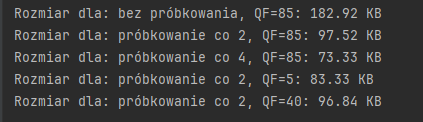
\includegraphics{Img/zad45_1.png}%
    }
    \caption{Logi konsoli opisujące rozmiary obrazów po kompresji (z różnymi parametrami)}
    \label{fig:zad45_1}
\end{figure}

\subsection*{Obraz po kompresji i dekompresji (z różnymi parametrami)}
\begin{figure}[H]
    \centering
    \resizebox{\columnwidth}{!}{%
        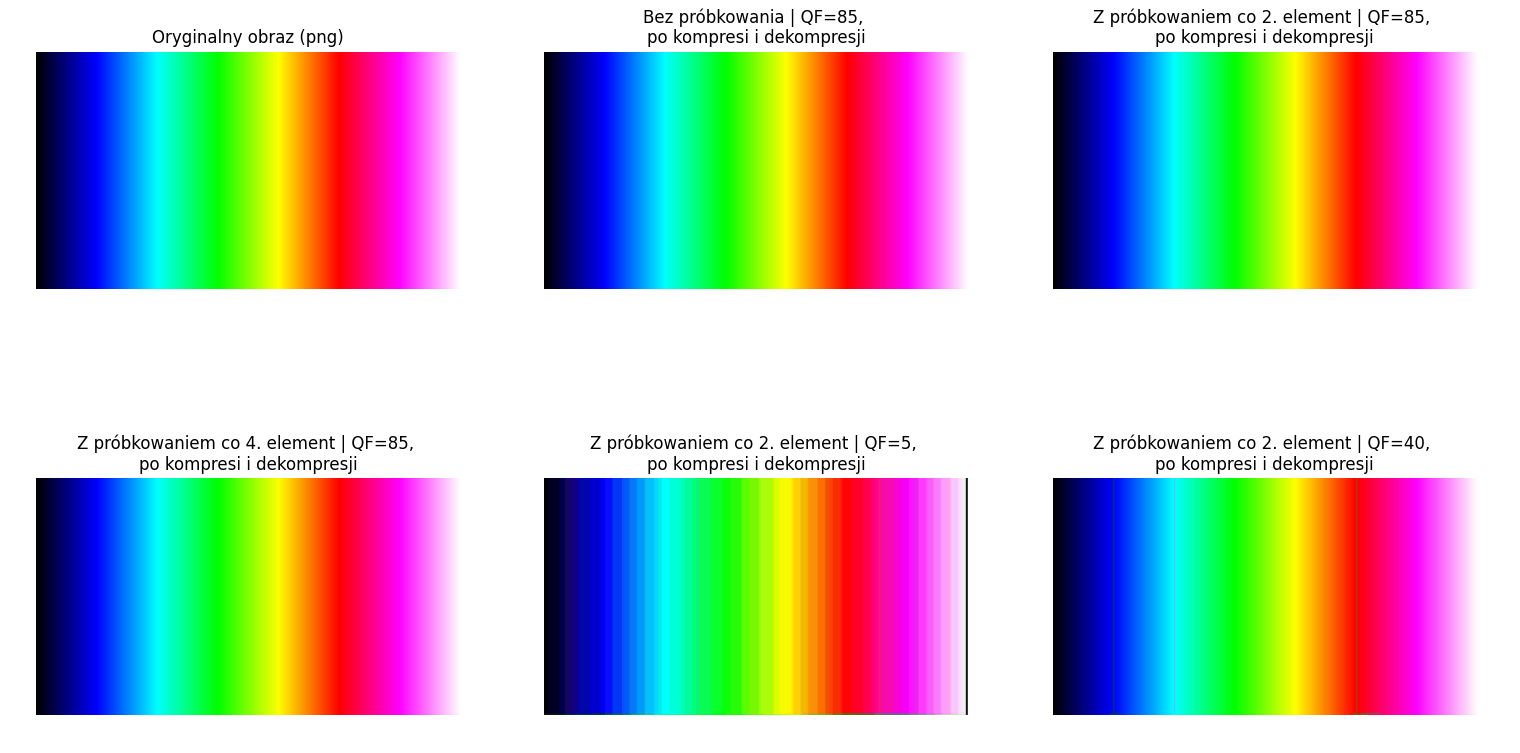
\includegraphics{Img/zad45.png}%
    }
    \caption{Prezentacja oryginalnego obrazu wraz z wariacjami po kompresji i dekompresji (z różnymi parametrami)}
    \label{fig:zad45}
\end{figure}

\subsection*{Wartości współczynnika MSE pomiedzy oryginalnym obrazem a obrazem po kompresji i dekompresji (z różnymi parametrami)}
\begin{figure}[H]
    \centering
    \resizebox{\columnwidth}{!}{%
        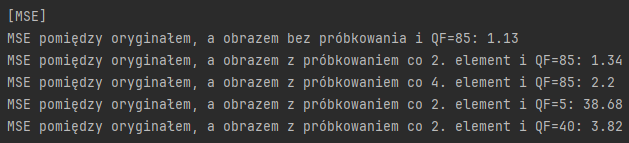
\includegraphics{Img/zad45_2.png}%
    }
    \caption{Logi konsoli prezentujące współczynniki MSE pomiedzy oryginalnym obrazem a obrazem po kompresji i dekompresji (z różnymi parametrami)}
    \label{fig:zad45_2}
\end{figure}

\section{Wnioski}
Podczas laboratorium pomyślnie zaimplementowałem algorytm JPEG.
Na podstawie wykonanych zadań zauważyłem, że wybór parametrów takich jak czynnik jakości (QF) czy technika
próbkowania ma znaczący wpływ na rozmiar i jakość obrazu.
\begin{itemize}
    \item Wraz ze wzrostem czynnika jakości (QF) rośnie jakość obrazu, ale maleje stopień kompresji (co za tym
          idzie, zwiększa się rozmiar obrazu).
    \item Technika próbkowania również wpływa na rozmiar obrazu. Wraz ze wzrostem stopnia próbkowania
          maleje rozmiar obrazu, ale rośnie utrata jakości.
\end{itemize}

\bibliographystyle{plainnat}
\bibliography{TexBase/Bibliography}

\end{document}